% =====================================================================
% File        : perulangan_matlab.tex
% Deskripsi   : Perulangan/iterasi (looping) di MATLAB: konsep loop,
%               for loop, while loop, dan apa saja yang bisa diulang
% =====================================================================
\documentclass[aspectratio=169,11pt]{beamer}
\usetheme{metropolis}
\usepackage[utf8]{inputenc}
\usepackage{amsmath,amssymb}
\usepackage{booktabs}
\usepackage{listings}
\usepackage{tikz}
\usetikzlibrary{positioning,arrows.meta,shapes.misc,shapes.geometric,matrix}

\definecolor{kolom}{RGB}{31,119,180}
\definecolor{baris}{RGB}{214,39,40}
\definecolor{kode}{RGB}{245,245,245}

% Kotak "Masalah / Dicari" di awal slide contoh
\newcommand{\masalah}[3]{%
  \noindent\colorbox{kolom!8}{\parbox{\dimexpr\linewidth-2\fboxsep\relax}{%
    \footnotesize\textbf{Data:} #1\\[1pt]
    \textbf{Masalah:} #2\\[1pt]
    \textbf{Dicari:} #3}}\par\vspace{0.35em}}

\lstset{
  language=Matlab,
  basicstyle=\ttfamily\small,
  backgroundcolor=\color{kode},
  keywordstyle=\color{kolom}\bfseries,
  commentstyle=\color{gray}\itshape,
  frame=single, rulecolor=\color{gray!40},
  columns=fullflexible, keepspaces=true,
  xleftmargin=4pt, xrightmargin=4pt,
  showstringspaces=false
}

\title{Perulangan/Iterasi (Looping)}
\subtitle{\texttt{for} loop dan \texttt{while} loop}
\author{Andreas Syaloom Kurniawan}
\institute{Faculty of Economics and Business, Universitas Gadjah Mada}
\date{}

\begin{document}

\maketitle

% ---------------------------------------------------------------------
\begin{frame}[fragile]{Kenapa kita butuh loop?}
\masalah{bilangan 2, 4, 6, 8, 10}
  {menghitung kuadrat setiap bilangan.}
  {$2^2, 4^2, \dots, 10^2$.}
\begin{columns}[T]
\column{0.32\textwidth}
\small Cara yang sudah kita bisa:
\begin{lstlisting}[basicstyle=\ttfamily\scriptsize]
x1 = 2^2;
x2 = 4^2;
x3 = 6^2;
x4 = 8^2;
x5 = 10^2;
\end{lstlisting}
\column{0.64\textwidth}
\small Perhatikan polanya:
\begin{itemize}
  \item Perhitungannya \alert{selalu sama}: bilangan dipangkatkan 2.
  \item Yang berubah \alert{hanya bilangannya}.
  \item Untuk 1.000 bilangan, cara ini butuh 1.000 baris.
\end{itemize}
\textbf{Ide loop:} tulis perhitungannya \textbf{sekali}, lalu minta MATLAB
mengulangnya untuk setiap bilangan.
\end{columns}
\end{frame}

% ---------------------------------------------------------------------
\begin{frame}{Tiga istilah dasar}
\small
\renewcommand{\arraystretch}{1.35}
\begin{tabular}{p{0.2\textwidth} p{0.72\textwidth}}
\toprule
Istilah & Arti \\
\midrule
\textbf{loop} & Struktur untuk mengulang suatu perhitungan (atau beberapa
  perhitungan) berkali-kali. \\
\textbf{pass} & Satu kali pengulangan. Loop yang berulang 5 kali punya
  5 pass. Sering juga disebut \emph{iterasi}. \\
\textbf{kondisi berhenti} & Aturan yang menentukan kapan loop selesai. \\
\bottomrule
\end{tabular}

\vspace{0.8em}
\textbf{Analogi: naik tangga.} Setiap anak tangga yang dinaiki adalah satu
\alert{pass}. Gerakannya selalu sama: angkat kaki, naik satu anak tangga. Kita
berhenti ketika sampai di lantai tujuan: itulah \alert{kondisi berhenti}.
\end{frame}

% ---------------------------------------------------------------------
\begin{frame}{Dua cara menentukan kapan berhenti}
\begin{columns}[T]
\column{0.48\textwidth}
\textbf{\texttt{for}: jumlah pass sudah diketahui}

\small Seperti mengabsen 30 mahasiswa satu per satu. Sebelum mulai, kita sudah
tahu akan ada tepat 30 panggilan.

\vspace{0.4em}
Contoh di ekonomi: simulasi model selama $T = 100$ periode.
\column{0.48\textwidth}
\textbf{\texttt{while}: ulangi selama kondisi benar}

\small Seperti mengaduk kopi \emph{selama} gulanya belum larut. Kita tidak tahu
berapa kali harus mengaduk; kita hanya terus mengecek.

\vspace{0.4em}
Contoh di ekonomi: iterasi mencari steady state sampai konvergen.
\end{columns}

\vspace{1em}
\centering
Pertanyaan kunci sebelum menulis loop:\\[0.2em]
\alert{``Apakah saya sudah tahu berapa kali harus mengulang?''}\\[0.2em]
\small Ya $\rightarrow$ \texttt{for} \qquad Tidak $\rightarrow$ \texttt{while}
\end{frame}

% ---------------------------------------------------------------------
\begin{frame}{Alurnya sama, yang berbeda siapa yang mengurus}
\centering
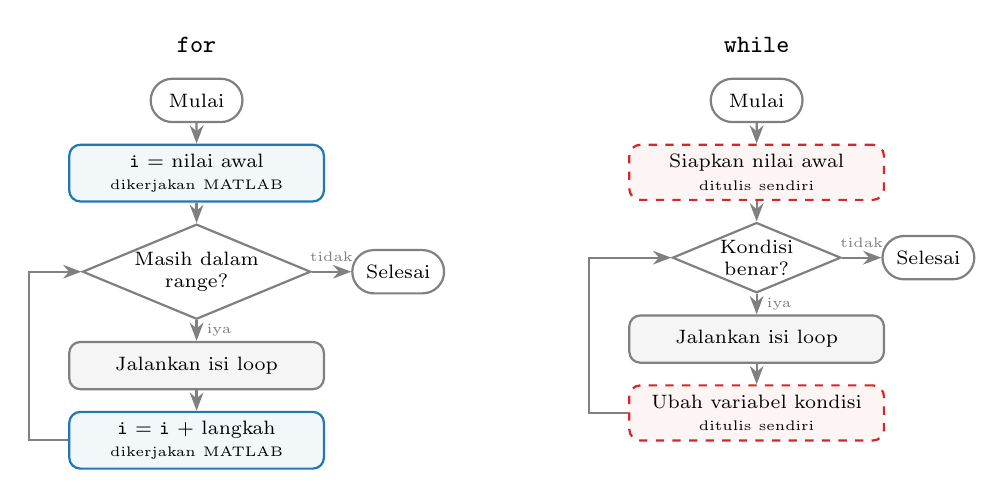
\begin{tikzpicture}[
  node distance=2.6mm and 6mm,
  >=Stealth,
  ujung/.style={draw=gray, thick, rounded rectangle, minimum height=5.5mm,
                minimum width=14mm, font=\scriptsize},
  isi/.style={draw=gray, fill=gray!8, thick, rounded corners,
              minimum height=6mm, text width=30mm, align=center, font=\scriptsize},
  auto/.style={draw=kolom, fill=kolom!6, thick, rounded corners,
               minimum height=7mm, text width=30mm, align=center, font=\scriptsize},
  manual/.style={draw=baris, fill=baris!5, thick, dashed, rounded corners,
                 minimum height=7mm, text width=30mm, align=center, font=\scriptsize},
  cek/.style={draw=gray, fill=white, thick, diamond, aspect=2.4, inner sep=0.5pt,
              font=\scriptsize, align=center},
  lab/.style={font=\tiny, text=gray}]
  % ---- for ----
  \node[font=\small\bfseries] (tf) {\texttt{for}};
  \node[ujung, below=2mm of tf] (a1) {Mulai};
  \node[auto, below=of a1] (b1) {\texttt{i} = nilai awal\\{\tiny dikerjakan MATLAB}};
  \node[cek, below=of b1] (c1) {Masih dalam\\range?};
  \node[isi, below=of c1] (d1) {Jalankan isi loop};
  \node[auto, below=of d1] (e1) {\texttt{i} = \texttt{i} + langkah\\{\tiny dikerjakan MATLAB}};
  \node[ujung, right=5mm of c1] (f1) {Selesai};
  \draw[->, thick, gray] (a1)--(b1); \draw[->, thick, gray] (b1)--(c1);
  \draw[->, thick, gray] (c1)--node[lab, right]{iya}(d1);
  \draw[->, thick, gray] (d1)--(e1);
  \draw[->, thick, gray] (c1)--node[lab, above]{tidak}(f1);
  \draw[->, thick, gray] (e1.west)--++(-5mm,0)|-(c1.west);
  % ---- while ----
  \node[font=\small\bfseries, right=62mm of tf] (tw) {\texttt{while}};
  \node[ujung, below=2mm of tw] (a2) {Mulai};
  \node[manual, below=of a2] (b2) {Siapkan nilai awal\\{\tiny ditulis sendiri}};
  \node[cek, below=of b2] (c2) {Kondisi\\benar?};
  \node[isi, below=of c2] (d2) {Jalankan isi loop};
  \node[manual, below=of d2] (e2) {Ubah variabel kondisi\\{\tiny ditulis sendiri}};
  \node[ujung, right=5mm of c2] (f2) {Selesai};
  \draw[->, thick, gray] (a2)--(b2); \draw[->, thick, gray] (b2)--(c2);
  \draw[->, thick, gray] (c2)--node[lab, right]{iya}(d2);
  \draw[->, thick, gray] (d2)--(e2);
  \draw[->, thick, gray] (c2)--node[lab, above]{tidak}(f2);
  \draw[->, thick, gray] (e2.west)--++(-5mm,0)|-(c2.west);
\end{tikzpicture}

\vspace{0.2em}
\footnotesize \textcolor{kolom}{\textbf{Kotak biru}} dikerjakan MATLAB secara
otomatis. \textcolor{baris}{\textbf{Kotak merah putus-putus}} harus kamu tulis
sendiri.
\end{frame}

% =====================================================================
\section{\texttt{for} Loop}
% =====================================================================

\begin{frame}[fragile]{Bahan dasar: range \texttt{m:s:n}}
\begin{columns}[T]
\column{0.42\textwidth}
\small Sebelum masuk ke loop, kenali dulu cara MATLAB membuat deretan angka.
\begin{lstlisting}[basicstyle=\ttfamily\footnotesize]
>> 2:2:10
ans =
     2     4     6     8    10
\end{lstlisting}
\footnotesize
\renewcommand{\arraystretch}{1.15}
\begin{tabular}{l l}
\texttt{m} & nilai awal (di sini 2) \\
\texttt{s} & langkah, ditambahkan tiap kali (2) \\
\texttt{n} & nilai akhir, batas atas (10) \\
\end{tabular}
\column{0.54\textwidth}
\footnotesize
\renewcommand{\arraystretch}{1.15}
\begin{tabular}{l l l}
\toprule
Ditulis & Hasil & Catatan \\
\midrule
\texttt{1:5} & \texttt{1 2 3 4 5} & langkah dihilangkan = 1 \\
\texttt{1:3:10} & \texttt{1 4 7 10} & 10 tepat terkena \\
\texttt{0:5:12} & \texttt{0 5 10} & 15 sudah melewati 12 \\
\texttt{10:-2:2} & \texttt{10 8 6 4 2} & langkah negatif: mundur \\
\texttt{2:2:5} & \texttt{2 4} & berhenti sebelum melewati 5 \\
\texttt{10:2:2} & \textit{kosong} & awal sudah melewati batas \\
\bottomrule
\end{tabular}

\vspace{0.6em}
\small \texttt{for} loop menjalankan \alert{satu pass untuk setiap angka}
dalam range. Jika isi range bisa ditebak, jumlah pass juga sudah diketahui.
\end{columns}
\end{frame}

% ---------------------------------------------------------------------
\begin{frame}[fragile]{Sintaks \texttt{for} dan contoh pertama}
\begin{columns}[T]
\column{0.5\textwidth}
\begin{lstlisting}[basicstyle=\ttfamily\normalsize]
for variable = m:s:n
    statement(s)
end
\end{lstlisting}
\small Dibaca: ``\textbf{untuk setiap} nilai \texttt{variable} di dalam
\texttt{m:s:n}, jalankan \texttt{statement(s)}.''
\begin{itemize}\footnotesize
  \item \texttt{variable} disebut \alert{loop index}; namanya bebas
        (\texttt{i}, \texttt{k}, \texttt{tahun}).
  \item Di setiap pass, MATLAB \alert{otomatis} mengisinya dengan angka
        berikutnya dari range.
  \item \texttt{end} menandai akhir bagian yang diulang.
\end{itemize}
\column{0.46\textwidth}
\begin{lstlisting}[basicstyle=\ttfamily\footnotesize]
for i = 1:3
    disp(i)
end
\end{lstlisting}
\begin{lstlisting}[basicstyle=\ttfamily\footnotesize]
     1
     2
     3
\end{lstlisting}
\footnotesize
\begin{tabular}{c c l}
\toprule
Pass & \texttt{i} & yang terjadi \\
\midrule
1 & 1 & tampilkan 1 \\
2 & 2 & tampilkan 2 \\
3 & 3 & tampilkan 3 \\
\bottomrule
\end{tabular}

\vspace{0.3em}
Range \texttt{1:3} berisi 3 angka, jadi ada 3 pass.
\end{columns}
\end{frame}

% ---------------------------------------------------------------------
\begin{frame}[fragile]{Menampilkan hasil: \texttt{disp}, bukan \texttt{print}}
\begin{columns}[T]
\column{0.5\textwidth}
\begin{lstlisting}[basicstyle=\ttfamily\footnotesize]
>> x = [4 16 36];
>> x                 % tanpa titik koma
x =
     4    16    36
>> disp(x)           % nilainya saja
     4    16    36
>> fprintf('%d ', x) % format sendiri
4 16 36
\end{lstlisting}
\column{0.46\textwidth}
\small
\begin{itemize}
  \item Di MATLAB, \texttt{print} dipakai untuk mencetak atau menyimpan
        \alert{figure} (grafik), bukan menampilkan isi variabel. Itu berbeda
        dengan \texttt{print} di Python.
  \item Baris yang diakhiri \texttt{;} tetap dijalankan, tetapi hasilnya
        \alert{tidak ditampilkan}.
  \item Di dalam loop, hilangkan \texttt{;} atau pakai \texttt{disp} jika ingin
        melihat nilai di setiap pass.
\end{itemize}
\end{columns}
\end{frame}

% ---------------------------------------------------------------------
\begin{frame}[fragile]{Contoh 1: kuadrat, tetapi hasilnya tertimpa}
\masalah{range \texttt{2:2:10}}
  {menghitung kuadrat setiap angka dengan loop.}
  {vektor berisi $4, 16, 36, 64, 100$.}
\begin{columns}[T]
\column{0.4\textwidth}
\begin{lstlisting}[basicstyle=\ttfamily\footnotesize]
for i = 2:2:10
    x = i^2;
end
x
\end{lstlisting}
\begin{lstlisting}[basicstyle=\ttfamily\footnotesize]
x =
   100
\end{lstlisting}
\column{0.56\textwidth}
\footnotesize
\begin{tabular}{c c c}
\toprule
Pass & \texttt{i} & isi \texttt{x} setelah pass \\
\midrule
1 & 2 & 4 \\
2 & 4 & 16 \\
3 & 6 & 36 \\
4 & 8 & 64 \\
5 & 10 & 100 \\
\bottomrule
\end{tabular}

\vspace{0.4em}
\small \texttt{x} hanya menampung \alert{satu angka}. Setiap pass menimpa
hasil pass sebelumnya, sehingga yang tersisa hanya hasil pass terakhir.
\end{columns}
\end{frame}

% ---------------------------------------------------------------------
\begin{frame}[fragile]{Contoh 1 (perbaikan): simpan hasil di posisinya sendiri}
\begin{columns}[T]
\column{0.4\textwidth}
\begin{lstlisting}[basicstyle=\ttfamily\footnotesize]
k = 0;      % posisi
for i = 2:2:10
    k = k + 1;
    x(k) = i^2;
end
x
\end{lstlisting}
\begin{lstlisting}[basicstyle=\ttfamily\footnotesize]
x =
     4    16    36    64   100
\end{lstlisting}
\column{0.56\textwidth}
\footnotesize
\begin{tabular}{c c c l}
\toprule
Pass & \texttt{i} & \texttt{k} & isi \texttt{x} setelah pass \\
\midrule
1 & 2 & 1 & \texttt{[4]} \\
2 & 4 & 2 & \texttt{[4 16]} \\
3 & 6 & 3 & \texttt{[4 16 36]} \\
4 & 8 & 4 & \texttt{[4 16 36 64]} \\
5 & 10 & 5 & \texttt{[4 16 36 64 100]} \\
\bottomrule
\end{tabular}

\vspace{0.4em}
\small
\begin{itemize}\footnotesize
  \item \texttt{k} naik 1 di setiap pass, sehingga tiap hasil masuk ke posisi
        baru: 1, 2, 3, 4, 5.
  \item Kenapa bukan \texttt{x(i)}? \texttt{i} bernilai 2, 4, 6, \dots{} Posisi
        1, 3, 5, \dots{} akan terisi 0 dan panjang \texttt{x} menjadi 10,
        bukan 5.
\end{itemize}
\end{columns}
\end{frame}

% ---------------------------------------------------------------------
\begin{frame}[fragile]{Versi tanpa loop, dan kapan loop tetap dibutuhkan}
\begin{columns}[T]
\column{0.48\textwidth}
\small Untuk perhitungan sederhana, MATLAB bisa menghitung satu vektor
sekaligus:
\begin{lstlisting}[basicstyle=\ttfamily\footnotesize]
>> x = (2:2:10).^2
x =
     4    16    36    64   100
\end{lstlisting}
\footnotesize Titik sebelum \texttt{\^} berarti operasi \alert{per elemen}.
Hasilnya sama dengan loop tadi dan biasanya lebih cepat.
\column{0.48\textwidth}
\small Loop tetap dibutuhkan ketika sebuah pass \alert{bergantung pada hasil
pass sebelumnya}, misalnya simulasi AR(1):
\[ y_t = 0.9\,y_{t-1} + \varepsilon_t \]
\begin{lstlisting}[basicstyle=\ttfamily\footnotesize]
T = 100;
y = zeros(T,1);       % preallocate
e = randn(T,1);
for t = 2:T
    y(t) = 0.9*y(t-1) + e(t);
end
\end{lstlisting}
\end{columns}
\end{frame}

% ---------------------------------------------------------------------
\begin{frame}[fragile]{Jebakan 1: \texttt{n} adalah batas, bukan nilai terakhir}
\begin{columns}[T]
\column{0.48\textwidth}
\begin{lstlisting}[basicstyle=\ttfamily\footnotesize]
for i = 2:2:5
    disp(i)
end
\end{lstlisting}
\begin{lstlisting}[basicstyle=\ttfamily\footnotesize]
     2
     4
\end{lstlisting}
\small Angka 6 sudah melewati 5, jadi loop berhenti setelah \alert{2 pass}.
\texttt{i} tidak pernah bernilai 5.
\column{0.48\textwidth}
\begin{lstlisting}[basicstyle=\ttfamily\footnotesize]
for i = 10:2:2
    disp(i)
end
\end{lstlisting}
\begin{lstlisting}[basicstyle=\ttfamily\footnotesize]
     (tidak ada output)
\end{lstlisting}
\small Range-nya kosong, jadi \alert{0 pass}: isi loop tidak pernah
dijalankan dan tidak ada error. Untuk menghitung mundur, langkahnya harus
negatif: \texttt{10:-2:2}.
\end{columns}
\end{frame}

% ---------------------------------------------------------------------
\begin{frame}[fragile]{Jebakan 2: mengubah loop index di dalam loop}
\begin{columns}[T]
\column{0.44\textwidth}
\begin{lstlisting}[basicstyle=\ttfamily\footnotesize]
for mama = 3:2:100
    mama = mama - 5
end
\end{lstlisting}
\footnotesize
\begin{tabular}{c c c}
\toprule
Pass & \texttt{mama} di awal & yang tercetak \\
\midrule
1 & 3 & $-2$ \\
2 & 5 & 0 \\
3 & 7 & 2 \\
$\vdots$ & $\vdots$ & $\vdots$ \\
49 & 99 & 94 \\
\bottomrule
\end{tabular}
\column{0.52\textwidth}
\small Kodenya \alert{jalan}, tetapi:
\begin{itemize}\footnotesize
  \item Perubahan \texttt{mama - 5} hanya berlaku \alert{sampai akhir pass}.
        Pass berikutnya tetap mengambil angka selanjutnya dari range.
  \item Jumlah pass tetap 49. Setelah loop selesai, \texttt{mama} bernilai 94.
  \item Editor MATLAB memberi \alert{peringatan oranye}: \emph{loop index is
        changed inside of a FOR loop}.
\end{itemize}
\vspace{0.3em}
\small\textbf{Kebiasaan yang aman:} biarkan loop index hanya menghitung pass,
lalu simpan hasil ke variabel lain, misalnya \texttt{y = mama - 5;}.
\end{columns}
\end{frame}

% ---------------------------------------------------------------------
\begin{frame}[fragile]{Latihan \texttt{for}}
\small Kerjakan dulu di kertas, lalu cek di MATLAB. Jawaban ada di akhir.
\begin{columns}[T]
\column{0.5\textwidth}
\begin{enumerate}
  \item Berapa jumlah pass pada \texttt{for i = 1:3:10}?
  \item Apa isi \texttt{x} setelah kode berikut?
\begin{lstlisting}[basicstyle=\ttfamily\footnotesize]
for i = 5:-1:3
    x = i;
end
\end{lstlisting}
\end{enumerate}
\column{0.46\textwidth}
\begin{enumerate}\setcounter{enumi}{2}
  \item Berapa nilai \texttt{k} setelah loop \texttt{2:2:10} pada contoh
        perbaikan selesai?
  \item Tulis loop untuk menyimpan $1^3, 2^3, \dots, 6^3$ ke dalam vektor
        \texttt{y}.
  \item Ubah contoh AR(1) agar menyimpan $y_t$ untuk koefisien $0.5$, lalu
        bandingkan \texttt{y(100)} kedua versi dengan \texttt{e} yang sama.
\end{enumerate}
\end{columns}
\end{frame}

% =====================================================================
\section{\texttt{while} Loop}
% =====================================================================

\begin{frame}[fragile]{Bahan dasar: kondisi, lalu sintaks \texttt{while}}
\begin{columns}[T]
\column{0.4\textwidth}
\small \texttt{while} bergantung pada \alert{kondisi}: pernyataan yang
jawabannya benar (\texttt{1}) atau salah (\texttt{0}).
\begin{lstlisting}[basicstyle=\ttfamily\footnotesize]
>> 5 <= 10
ans =
  logical
   1
\end{lstlisting}
\footnotesize Sebaliknya, \texttt{12 <= 10} menghasilkan \texttt{0}.
\column{0.56\textwidth}
\begin{lstlisting}[basicstyle=\ttfamily\small]
while kondisi
    statement(s)
end
\end{lstlisting}
\small Dibaca: ``\textbf{selama} kondisi masih benar, jalankan
\texttt{statement(s)}.'' Berbeda dengan \texttt{for}, ada \alert{tiga hal} yang kamu urus sendiri:
\begin{enumerate}\footnotesize
  \item \textbf{Siapkan}: beri nilai awal sebelum loop.
  \item \textbf{Cek}: kondisi dicek \emph{sebelum} setiap pass.
  \item \textbf{Ubah}: ubah variabel kondisi di dalam loop; tanpa ini loop
        tidak pernah berhenti.
\end{enumerate}
\end{columns}
\end{frame}

% ---------------------------------------------------------------------
\begin{frame}[fragile]{Contoh 2: kuadrat yang sama, ditulis dengan \texttt{while}}
\begin{columns}[T]
\column{0.42\textwidth}
\begin{lstlisting}[basicstyle=\ttfamily\footnotesize]
i = 2;              % siapkan
k = 0;
while i <= 10       % cek
    k = k + 1;
    x(k) = i^2;
    i = i + 2;      % ubah
end
x
\end{lstlisting}
\begin{lstlisting}[basicstyle=\ttfamily\footnotesize]
x =
     4    16    36    64   100
\end{lstlisting}
\column{0.54\textwidth}
\footnotesize
\begin{tabular}{c c c c c}
\toprule
Pass & \texttt{i} & \texttt{i <= 10}? & \texttt{x(k)} & \texttt{i} baru \\
\midrule
1 & 2 & benar & 4 & 4 \\
2 & 4 & benar & 16 & 6 \\
3 & 6 & benar & 36 & 8 \\
4 & 8 & benar & 64 & 10 \\
5 & 10 & benar & 100 & 12 \\
-- & 12 & \textcolor{baris}{salah} & \multicolumn{2}{l}{berhenti} \\
\bottomrule
\end{tabular}

\vspace{0.4em}
\small Hasilnya sama dengan versi \texttt{for}. Bedanya, \texttt{i = i + 2}
\alert{ditulis sendiri}, sedangkan di \texttt{for} MATLAB yang
mengerjakannya.
\end{columns}
\end{frame}

% ---------------------------------------------------------------------
\begin{frame}[fragile]{Jebakan: infinite loop dan 0 pass}
\begin{columns}[T]
\column{0.48\textwidth}
\textbf{Baris ``ubah'' terlupa}
\begin{lstlisting}[basicstyle=\ttfamily\footnotesize]
i = 2;
while i <= 10
    x = i^2;
    % i = i + 2;   (terlupa)
end
\end{lstlisting}
\small Di setiap pass \texttt{i} tetap 2, sehingga \texttt{2 <= 10} selalu
benar dan loop tidak pernah berhenti: \alert{infinite loop}. Hentikan dengan
\textbf{Ctrl+C} di Command Window.
\column{0.48\textwidth}
\textbf{Kondisi sudah salah sejak awal}
\begin{lstlisting}[basicstyle=\ttfamily\footnotesize]
i = 12;
while i <= 10
    x = i^2;
    i = i + 2;
end
x
\end{lstlisting}
\begin{lstlisting}[basicstyle=\ttfamily\scriptsize, deletekeywords={function}]
Unrecognized function or variable 'x'.
\end{lstlisting}
\small Kondisi dicek \alert{sebelum} pass pertama. Karena \texttt{12 <= 10}
salah, isi loop tidak pernah dijalankan (0 pass), sehingga \texttt{x} tidak
pernah dibuat.
\end{columns}
\end{frame}

% ---------------------------------------------------------------------
\begin{frame}[fragile]{Contoh 3: iterasi sampai konvergen}
\masalah{tebakan awal $x_0 = 1$, rumus perbaikan $x_{\text{baru}} = \tfrac12\left(x + \tfrac{2}{x}\right)$}
  {memperbaiki tebakan berulang kali sampai perubahannya sangat kecil.}
  {$\sqrt{2}$, dengan toleransi $10^{-8}$.}
\begin{columns}[T]
\column{0.44\textwidth}
\begin{lstlisting}[basicstyle=\ttfamily\scriptsize]
x = 1;
err = 1;
while err > 1e-8
    x_baru = 0.5*(x + 2/x);
    err = abs(x_baru - x);
    x = x_baru;
end
x
\end{lstlisting}
\column{0.52\textwidth}
\footnotesize
\begin{tabular}{c l l l}
\toprule
Pass & \texttt{x} & \texttt{err} & \texttt{err > 1e-8}? \\
\midrule
1 & 1.500000 & 0.5 & benar \\
2 & 1.416667 & 0.0833 & benar \\
3 & 1.414216 & 0.00245 & benar \\
4 & 1.414214 & $2.12\times10^{-6}$ & benar \\
5 & 1.414214 & $1.59\times10^{-12}$ & \textcolor{baris}{salah} \\
\bottomrule
\end{tabular}
\begin{itemize}\footnotesize
  \item Tidak ada loop index; yang menghentikan loop adalah \texttt{err}
        yang makin kecil. Jumlah pass (5) baru diketahui setelah selesai.
  \item Pola yang sama dipakai untuk mencari steady state atau value function
        iteration.
\end{itemize}
\end{columns}
\end{frame}

% ---------------------------------------------------------------------
\begin{frame}[fragile]{Pengaman: batas iterasi dan \texttt{break}}
\begin{columns}[T]
\column{0.48\textwidth}
\textbf{Batas iterasi}

\small Jika belum tentu konvergen, tambahkan penghitung agar loop pasti
berhenti.
\begin{lstlisting}[basicstyle=\ttfamily\scriptsize]
iter = 0;
while err > 1e-8 && iter < 1000
    % ... isi loop ...
    iter = iter + 1;
end
if iter == 1000
    warning('Belum konvergen')
end
\end{lstlisting}
\column{0.48\textwidth}
\textbf{\texttt{break}}

\small Menghentikan loop saat itu juga; berlaku untuk \texttt{for} maupun
\texttt{while}.
\begin{lstlisting}[basicstyle=\ttfamily\scriptsize]
for i = 1:100
    if i^2 > 50
        break
    end
    disp(i)
end
\end{lstlisting}
\small Menampilkan 1 sampai 7, lalu berhenti karena $8^2 = 64 > 50$.
\end{columns}
\end{frame}

% ---------------------------------------------------------------------
\begin{frame}[fragile]{Latihan \texttt{while}}
\small Kerjakan dulu di kertas, lalu cek di MATLAB. Jawaban ada di akhir.
Koma memisahkan perintah dalam satu baris.
\vspace{0.3em}
\begin{columns}[T]
\column{0.48\textwidth}
\begin{enumerate}
  \item Berapa nilai akhir \texttt{i} dan jumlah pass?
\begin{lstlisting}[basicstyle=\ttfamily\scriptsize]
i = 1;  while i < 20,  i = i*3;  end
\end{lstlisting}
  \item Berapa nilai akhir \texttt{i}?
\begin{lstlisting}[basicstyle=\ttfamily\scriptsize]
i = 10;  while i > 0,  i = i - 3;  end
\end{lstlisting}
\end{enumerate}
\column{0.48\textwidth}
\begin{enumerate}\setcounter{enumi}{2}
  \item Berapa pass yang dijalankan?
\begin{lstlisting}[basicstyle=\ttfamily\scriptsize]
i = 5;  while i < 5,  i = i + 1;  end
\end{lstlisting}
  \item Apa masalahnya, dan bagaimana memperbaikinya?
\begin{lstlisting}[basicstyle=\ttfamily\scriptsize]
n = 1;  while n < 10,  disp(n),  end
\end{lstlisting}
\end{enumerate}
\end{columns}
\end{frame}

% =====================================================================
\section{Apa Saja yang Bisa Diulang}
% =====================================================================

\begin{frame}[fragile]{Isi loop tidak terbatas pada satu rumus (1)}
\small Apa pun yang ditulis di antara baris loop dan \texttt{end} dijalankan
ulang di setiap pass.
\vspace{0.3em}
\begin{columns}[T]
\column{0.32\textwidth}
\textbf{Indeks atau posisi}
\begin{lstlisting}[basicstyle=\ttfamily\scriptsize]
for k = 1:5
    x(k) = 2*k;
end
% x = [2 4 6 8 10]
\end{lstlisting}
\column{0.32\textwidth}
\textbf{Variabel yang diperbarui}
\begin{lstlisting}[basicstyle=\ttfamily\scriptsize]
total = 0;
for i = 1:5
    total = total + i;
end
% total = 15
\end{lstlisting}
\column{0.32\textwidth}
\textbf{Function}
\begin{lstlisting}[basicstyle=\ttfamily\scriptsize]
f = @(t) 3*t + 1;
for i = 1:3
    y(i) = sqrt(i) + f(i);
end
\end{lstlisting}
\end{columns}
\vspace{0.4em}
\footnotesize \textbf{Indeks}: hasil tiap pass masuk ke posisi berbeda.
\textbf{Variabel yang diperbarui}: nilai baru dihitung dari nilai lama
(akumulasi). \textbf{Function}: function bawaan maupun buatan sendiri bisa
dipanggil di setiap pass.
\end{frame}

% ---------------------------------------------------------------------
\begin{frame}[fragile]{Isi loop tidak terbatas pada satu rumus (2)}
\begin{columns}[T]
\column{0.32\textwidth}
\textbf{Kondisi di dalam loop}
\begin{lstlisting}[basicstyle=\ttfamily\footnotesize]
for i = 2:2:6
    if i > 4
        x(i/2) = i^2;
    else
        x(i/2) = i^2 - 1;
    end
end
% x = [3 15 36]
\end{lstlisting}
\column{0.32\textwidth}
\textbf{Loop di dalam loop}
\begin{lstlisting}[basicstyle=\ttfamily\footnotesize]
for r = 1:3
    for c = 1:3
        A(r,c) = r*c;
    end
end
% tabel perkalian 3x3
\end{lstlisting}
\column{0.32\textwidth}
\textbf{Daftar nilai bebas}
\begin{lstlisting}[basicstyle=\ttfamily\footnotesize]
for v = [3 7 1]
    disp(v*10)
end
for kota = ["Jogja" "Solo"]
    disp(kota)
end
\end{lstlisting}
\end{columns}
\vspace{0.4em}
\footnotesize Loop juga dipakai untuk membaca banyak file, membuat banyak
grafik, atau menjalankan simulasi dengan parameter berbeda-beda.
\end{frame}

% ---------------------------------------------------------------------
\begin{frame}{Ringkasan}
\centering\small
\renewcommand{\arraystretch}{1.3}
\begin{tabular}{l l l}
\toprule
 & \texttt{for} & \texttt{while} \\
\midrule
Dipakai ketika & jumlah pass sudah diketahui & jumlah pass belum diketahui \\
Berhenti karena & angka di range habis & kondisi menjadi salah \\
Yang memperbarui & MATLAB, otomatis & kamu, di dalam loop \\
Risiko utama & range salah tulis (0 pass) & infinite loop \\
Contoh ekonomi & simulasi $T = 100$ periode & iterasi sampai konvergen \\
\bottomrule
\end{tabular}

\vspace{0.8em}
\raggedright
\begin{itemize}
  \item Simpan hasil tiap pass di posisinya sendiri (\texttt{x(k)}), jika
        tidak hasilnya \alert{tertimpa}.
  \item Jangan mengubah loop index \texttt{for} di dalam loop.
  \item Di \texttt{while}: \alert{siapkan, cek, ubah}; tambahkan batas iterasi
        jika belum tentu konvergen.
\end{itemize}
\end{frame}

% ---------------------------------------------------------------------
\begin{frame}[fragile]{Jawaban latihan \texttt{for}}

\begin{enumerate}\small
  \item 4 pass: \texttt{i} bernilai 1, 4, 7, 10.
  \item \texttt{x = 3}. Loop menghitung mundur 5, 4, 3; karena \texttt{x}
        tanpa indeks, hanya nilai pass terakhir yang tersisa.
  \item \texttt{k = 5}, sama dengan jumlah pass.
  \item Salah satu jawaban (di sini \texttt{y(i)} aman karena \texttt{i} =
        1, 2, 3, \dots):
\begin{lstlisting}[basicstyle=\ttfamily\scriptsize]
for i = 1:6
    y(i) = i^3;    % [1 8 27 64 125 216]
end
\end{lstlisting}
  \item Ganti \texttt{0.9} menjadi \texttt{0.5} dan simpan ke vektor lain.
        Dengan koefisien lebih kecil, guncangan masa lalu memudar lebih cepat.
\end{enumerate}
\end{frame}

% ---------------------------------------------------------------------
\begin{frame}[fragile]{Jawaban latihan \texttt{while}}

\begin{enumerate}\small
  \item \texttt{i = 27}, 3 pass: $1 \to 3 \to 9 \to 27$, lalu
        \texttt{27 < 20} salah.
  \item \texttt{i = -2}, setelah 4 pass: $10 \to 7 \to 4 \to 1 \to -2$.
        Loop baru berhenti setelah kondisi salah, sehingga nilai akhir bisa
        melewati 0.
  \item 0 pass. \texttt{5 < 5} sudah salah sebelum pass pertama.
  \item Infinite loop: \texttt{n} tidak pernah berubah. Perbaikan:
\begin{lstlisting}[basicstyle=\ttfamily\scriptsize]
n = 1;
while n < 10
    disp(n)
    n = n + 1;
end
\end{lstlisting}
\end{enumerate}
\end{frame}

\end{document}
